%!TeX root = thesis-main.tex
\newcommand{\casename}[0]{{\sc{}FloodWatch}}


\newcommand{\revise}[1]{{#1}}
\newcommand{\revisetwo}[1]{{#1}}


\chapter[Dynamic Decentralization Domains]{Dynamic Decentralization Domains for \acf{cpsw}}\label{chap:eng:decentralization}%\mtcaddchapter
\minitoc% Creating an actual minitoc
Edge computing
 and related scenarios
 like \acp{cpsw}
 promote a vision of
 distributed computational systems 
 deeply integrated with
 humans and environments.
% 
% Such systems
%  will be characterized
%  by countless agents
%  requesting and/or supporting
%  resilient execution of applications
%  and services.
%
The complexity and volume in terms of devices, communications, failures, and change,
 are pushing the adoption of paradigms 
 that can %embrace these challenges
%  to
 adequately address both functional
 and non-functional of \ac{cpsw} that concerns of:
\begin{itemize}
  \item \emph{decentralization} for scalability and delegation;
  \item \emph{autonomic computing} and \emph{self-organization}~\cite{DBLP:journals/computer/KephartC03} for operational effectiveness and adaptation;
  \item \emph{in-network processing} for latency reduction and infrastructural autonomy; and
  \item \emph{collective computing}~\cite{DBLP:journals/eaai/CasadeiVAPD21} for coordination and collaboration.
\end{itemize}

Specifically, they form the platform % hardware and platforms 
 upon which several concurrent
 \emph{\acp{dcp}} 
 would run, carrying on transient activities
 by self-organized continuous computation and communication. %steps
%
The goal of a \ac{dcp} is to identify dynamic regions of the computational environment (regions of ``space'') where
situations of interest occur,
monitor their evolution,
and reactively trigger distributed actions to signal events,
remedy problems,
or control the phenomenon.
%
Hence, \acp{dcp}
 are generated
 to satisfy a request,
 handle an event, or 
 execute a collective task;
 they opportunistically spread (resp. shrinks)
 to gather (resp. release) resources/workers
 or cover (resp. uncover) regions of interest;
 they may perform 
 distributed sensing and actuation;
eventually, they may vanish once the activity is done.
 
In this chapter, 
 we address the problem of capturing the right abstractions for modelling \acp{dcp},
 abstracting from the specific communication technologies, 
 taking inspiration from the analogous 
 the approach taken in map-reduce frameworks for big data, 
 where the declarative concept of \emph{stream} is adopted.
%
and propose the concepts of \emph{concurrent collective tasks} 
 and \emph{decentralization domains}, % and \emph{region partitioning}, 
 which can be exploited in combination to provide distributed situated recognition and action.
%
\section{Motivation}\label{sec:motiv}

\acp{cpsw} are increasingly tasked with monitoring and acting upon dynamically changing environments, 
 often without the availability of a central coordinator.% Examples of such systems include crowd tracking and steering, environmental monitoring for landslides, flooding, and fires, and the coordination of robot swarms.

The recurrent approach in computer/software engineering 
 to manage such complexity is to adopt various \emph{levels} of abstractions 
 and mechanisms that encapsulate coherent sets of problems and solutions. 
This work aims to simplify the programming of these complex systems by enabling the user to express high-level goals, 
 without having to fully specify the \emph{how}. 
 This allows lower-level components to handle issues such as dynamicity, failure, and heterogeneity.

As an analogy, consider database management systems: 
 SQL queries express what data needs to be retrieved, while the system itself determines the most efficient way to fulfill the request. 
 The ultimate objective is to apply this principle to self-organizing systems, primarily to realize decentralized situation recognition and action.

\section{Decentralized situation recognition and action: a case study}
\label{decentralized-sr}
A \ac{cpsw} system
 should ideally determine autonomously
 \emph{what} has to be done,
 \emph{when},
 \emph{where},
 by \emph{whom},
 and \emph{how}.
%
The critical problem is setting up 
a \emph{decentralized process
for adaptive situation recognition
and situated action}.
%
The system 
 should organize to
 monitor the environment
 for situations
 requiring intervention;
 then, 
 the intervention should
%  be organized
%  and carried out to
 pursue
 the desired state of affairs.
%
These two phases do not need to be sequential but can be performed continuously in a feedback loop, gradually steering the system towards a correct and stable configuration.
%
Also, the system should \emph{opportunistically} 
  exploit available resources
  accordingly to the current context and goals---which may change dynamically.
%
Also,
we cannot assume the existence of a centralized coordinator
 such as the cloud,
which is usually relied upon in classic approaches.
 
As an example and case study throughout the paper,
consider a large-scale flood warning system,
which we call \casename{},
fully developed (in simulation) in \Cref{sec:eval}.
%
We want to monitor the rain intensity to pre-alert the public safety organizations close to areas at a \emph{risk} of floods.
%
The tracked phenomenon is spatially and temporally hard to predict with a fine-enough grain
(data from the NOAA\footnote{https://www.noaa.gov/} has, at best, zip-code granularity):
at a single-city level,
we could perform better by promptly reacting to specialized sensor readings.
%
However, the information provided by individual sensors is too fragile,
as the risk depends on the rain intensity in the surroundings and not just on the specific spot
(e.g., coastal zones with steep elevation profiles could suffer floods even with light rain,
if the close-by higher-altitude zone is being hit hard).
%
Pre-defining areas
(using pre-existing altimetric and structural knowledge)
helps, but this strategy misses out on essential information:
how the underlying phenomenon is behaving.
%
Indeed, areas should be formed ad-hoc considering the city structure and rain distribution,
% build ad-hoc sensing areas,
and leveraged to perform on-the-fly situation recognition and response.

This approach is practical whenever there are phenomena with non-strictly-local effects,
irregularly shaped in space,
and/or hard-to-predict at a fine grain.

\subsection{Requirements and abstractions}
Given the high-level vision and goals discussed in the previous sections, and with the help of \casename{},
 we delineate some \revisetwo{\emph{needs}
 together with \emph{abstractions} and corresponding \emph{requirements}, for a programming model 
 aimed at decentralized situation recognition and action.
 }
%  in \ac{iot} systems.
%
%\begin{enumerate}[label=\textbf{S.\arabic*}]
%\item[\enlabel{req-concurrency}{R1})] 

\subsubsection{\reqlabel{req-concurrency}{R1} Concurrent collective task execution.} 
%
In \casename{},
there is the need to coordinate
  a system that spans large geographical areas,
  hence leveraging \acp{dcp} for sensing, computation, and actuation
  at a collective level.
%
 One may also devise a more complex case study and platform
  for environmental monitoring
  where there is a distributed process for \casename{},
  another process for critical infrastructure monitoring,
 waste management,
 surveillance, etc.;
 these processes may run independently or,
 possibly,
 interact.

In general, most complex systems
 is not limited to a single activity
 but usually involve several activities running concurrently.
%
Furthermore,
these activities could be \emph{collective}, i.e.,
involve a collaboration of multiple agents with partial perception of the environment.
%We call each concurrent collective task instance a \emph{\ac{oca}}.
We call these \emph{\acp{cct}},
 which express activities that
 may \emph{overlap} in the system
 (a device may partake in multiple \acp{cct} simultaneously).
%
Notice that \acp{cct} may 
 have a limited and dynamic domain:
 a subset of devices in the system
 (sometimes also called \emph{team} or \emph{ensemble})
 which may change over time.

%\item[\enlabel{req-flexible-dec}{R2})] 
\subsubsection{\reqlabel{req-flexible-dec}{R2} Flexible and adaptive decentralization.} 
%
\casename{}
is centred on organizing distributed sensing and actuation
according to both the environment structure and the current rainfall.
%
Generally speaking, 
 strategies that are too fine-grained or too coarse-grained tend to be sub-optimal:
 in the former case,
non-local information is not considered,
possibly resulting in a lack of coherence and global inefficiency;
 in the latter case, 
 the system may fail to adequately recognize 
 specific contexts that should be handled ad-hoc.
%
In \casename{}, 
 warnings should be delivered 
 in the surroundings of risky areas,
 but not too broadly.

Many systems, indeed~\cite{DBLP:journals/fgcs/PianiniCVN21},
often need abstractions capturing an ``adaptive''
\emph{spatial divide-and-conquer}
principle through which a problem in space
% (e.g., situation recognition on a smart city)
is split into parts (or regions)
that
% dynamically and
opportunistically adapt according to the context.
% and partial results.
We call each region a \emph{\ac{dd}} since it represents a non-overlapping bounded subsystem of a \ac{cct}.
%
Multiple \acp{dd} can also \emph{compete} to gather resources exclusively within the domain defined by a \ac{cct}
(at whose level cross-domain interaction could happen, instead).

\subsubsection{\reqlabel{req-feedback}{R3} Feedback-regulated activity within decentralized domains.}
%
In \casename{}, each region
 should sense the water level and altitude,
 process data,
 and decide region-local actions such as alerting.
%
In a system for computational resource management,
 each region
 might collect resource advertisements and requests,
 compute assignments,
 and publish assignments
 while also monitoring and handling the activity progress.

In general, \acp{dd} are expected to autonomously carry out distributed sensing activities,
 followed by processing and decision-making,
which may trigger actions 
 affecting the environment
 (cf. actuations, for a kind of indirect feedback)
 or spawning new \acp{cct} (e.g., to connect with other services).
%
Often, in order to simplify and guarantee consistency at the level of \acp{dd}, 
decisions might be taken centrally in a \ac{dd} 
 by a leader. 
This could also be seen as a feedback loop: contributions are collected at the leader,
 the leader performs the decision-making
 and spreads the decisions which are then carried out,
 producing new data to be gathered and so on.

\subsubsection{Summary of requirements.}
\begin{figure*}
  \centering
  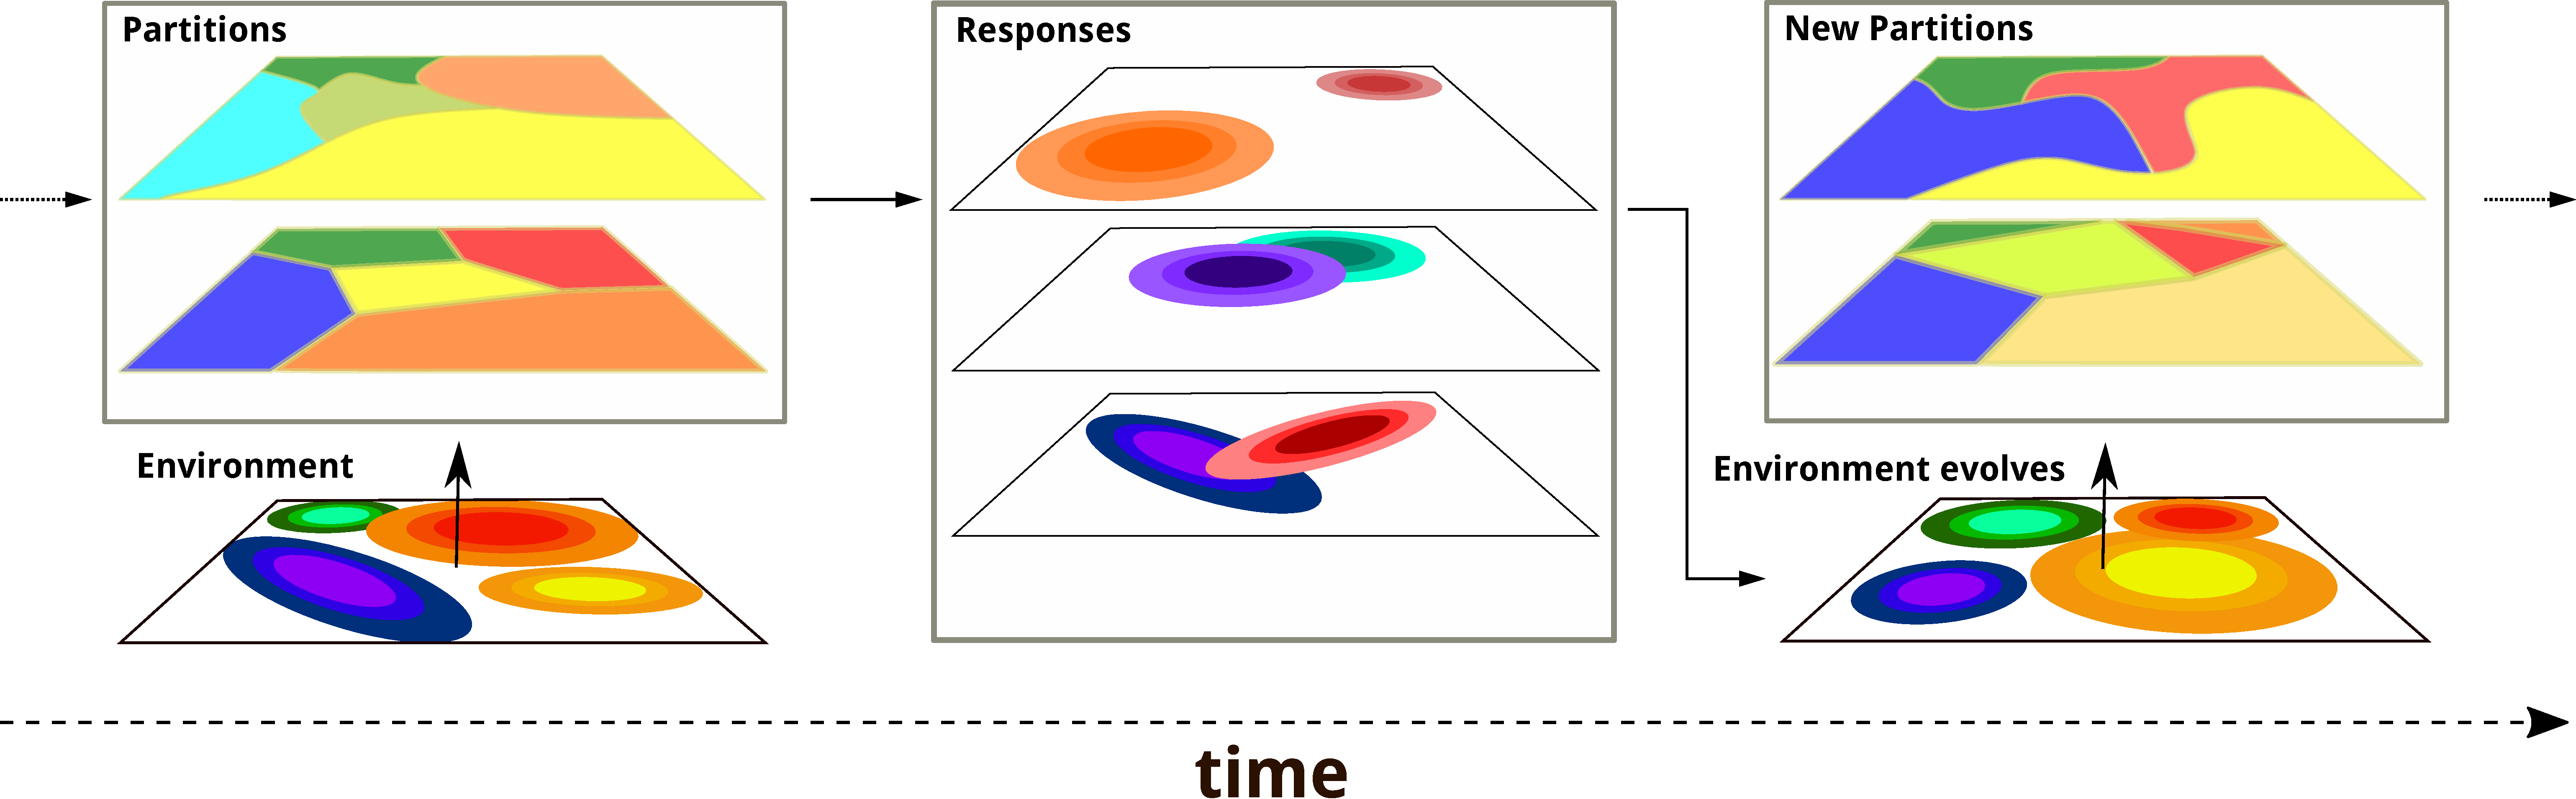
\includegraphics[width=\linewidth]{papers/ieee2022/img/approach-images/action-with-multilayer.pdf}
  \caption[Overview of the dynamic decentralization domains approach]{
    Overview of the proposed approach.
    The projected squares represent environments,
    with colours denoting environmental phenomena. % in terms e.g. of measured data or computed data associated to spatial locations.
    %Elements in gray boxes are software components,
    %whereas those outside denote real-world phenomena.
    Time flows left to right.
    The proposed system tracks spatial phenomena
    by partitioning the space in non-overlapping regions that agree on a measure,
    which is then leveraged to enact (multiple) spatially-bound responses
    that can % potentially cover only part of the space,
    overlap or compete.
    Contextual (induced or natural) changes
    %may lead to a change in the environment,
    are tracked by evolving (reshaping, deleting, or creating) the partitions.
  }
  \label{fig:high-level-description}
\end{figure*}

The rationale of the above requirements %, %in a nutshell,
 is to promote abstractions 
 supporting concurrent, system-spanning, and possibly overlapping activities (\ref{req-concurrency}),
 dynamic creation and maintenance of non-overlapping regions (\ref{req-flexible-dec}),
 and 
 internal loops of regional situation recognition and action
 (\ref{req-feedback}).
 \Cref{fig:high-level-description} summarizes these ideas.
\begin{comment}
\subsection{Related problem}

%\meta{
%*) State of the art addressed similar problems... -- we should both survey work of others, and then our recent works pertinent to what we are going to propose.
%% NB: we can have at max 20 bib refs
%}
%DBLP:journals/eaai/CasadeiVAPD21,DBLP:journals/fgcs/PianiniCVN21,DBLP:journals/computer/BealPV15,DBLP:journals/jlap/ViroliBDACP19

The
% declarative and macro-level
stance
 by which the behaviour of a whole system
 is expressed as a single program
 is shared by paradigms
 like
 macro-programming~\cite{DBLP:journals/csur/MottolaP11},
field-based computing~\cite{DBLP:journals/jlap/ViroliBDACP19},
 spatial computing~\cite{DBLP:books/daglib/0029568}, 
and
aggregate computing~\cite{DBLP:journals/computer/BealPV15}.
%
The programming model that we provide 
 is best understood as a higher-level wrapper
 on aggregate and field-based computations.
%  ,
% hiding details of the low-level constructs of their core languages~\cite{DBLP:journals/jlap/ViroliBDACP19}.
%  which are based on core languages~\cite{DBLP:journals/jlap/ViroliBDACP19} made of low-level constructs
%  such as \texttt{nbr} for interaction with neighbors and \texttt{rep} for local state management.

These approaches provide means
 for expressing \emph{collective} tasks and processes~\cite{DBLP:journals/tetc/ScekicSVRTMD20,DBLP:journals/eaai/CasadeiVAPD21}
 performed by \emph{ensembles}~\cite{DBLP:journals/computer/BuresPKTH16}
 of devices.
%
From~\cite{DBLP:journals/eaai/CasadeiVAPD21},
 we reuse the idea of \revise{\emph{aggregate processes}, i.e.,}
 computations 
 that spring out,
 spread, shrink, and vanish to express transient collective operations.
%  ---simplifying it by hiding to the programmer the complexity of propagation dynamics and structuring their usage by combination with exclusive domains.
%
\revise{
\acp{cct} can be thought of as a generalization of aggregate  
processes,
 and also differ from \emph{collective-based tasks}~\cite{DBLP:journals/tetc/ScekicSVRTMD20} which are based on orchestration.
}

The programming model covered in this article
is also related to \emph{\ac{scr}}~\cite{DBLP:journals/fgcs/PianiniCVN21},
a design pattern
% aiming to 
% solve distributed sensing and load balancing issues
%  in large-scale systems
% through a
promoting divide-and-conquer through dynamic feedback-regulated regional partitioning process.
% %
% The reader can refer to \cite{DBLP:journals/fgcs/PianiniCVN21} for a comprehensive survey of works and domains
% (ranging from \acp{wsn} and \ac{iot} to edge computing and swarm robotics)
% exploiting various forms of regional partitioning.
%
% In~\cite{DBLP:journals/fgcs/PianiniCVN21},,
%  it is shown that it is indeed a pattern
%  used in a variety of contexts ranging from
%  \acp{wsn} and \ac{iot} to edge computing and swarm robotics.
%
More generally,
the  importance of structured communities
in multi-agent systems
is witnessed by the sheer number of
\emph{organizational paradigms}~\cite{DBLP:journals/ker/HorlingL04}.
%
The abstractions presented in this paper 
 sit at a higher level % of abstraction
 and may be seen as implementatively exploiting \ac{scr} and organizational patterns %at the implementation level
 to solve the problem of decentralized situation recognition and action.
%
\revise{
Overall, the contribution of this work
 lies primarily in the \emph{combination}
 of the discussed abstractions into a simple but effective \ac{api}.
}
\end{comment}
\section{Dynamic Decentralization Domains in Practice}\label{sec:contrib}
\label{ssec:reqs-to-api}

From the previous discussion,
\revise{we further refine the}
requirements and extrapolate the design elements of an \ac{api}
supporting the decentralized computation we need:
%

\begin{itemize}
\item concerning \acp{cct} (cf. \ref{req-concurrency})
	\begin{itemize}
    \item we use a \ac{cct} to model a collective sensing task partitioned into multiple \emph{sensing domains} (i.e. \acp{dd}),
    where each sensing domain has a \emph{centre} and an \emph{extension} in space;
%    \meta{a CC model a DD? should improve on the relationship between the two}
    \item both the extension in space and the centre can change dynamically to improve the way the underlying phenomenon is being tracked,
    through selection of an appropriate leading node,
    definition of a metric (which can be other than the spatial distance),
    and definition of a granularity.
	\end{itemize}
\item concerning partitioning into \acp{dd} (cf. \ref{req-flexible-dec}) and activity within a \ac{dd} (cf. \ref{req-feedback})
    \begin{itemize}
    \item sensing domains for a single measure must not overlap,
    to avoid duplicate sampling and undesired interference
    (overlapping can be achieved through multiple \acp{cct},
    or by using a mixed custom metric);
%    \meta{a small comment on why?}
    \item inside a single sensing domain, a strategy is defined to collect the sensor readings;
    \item the decentralized sensing will output the collectively-sensed result and
      the identifier of the device closer to the area centre;
    \item the set of actions/actuations to perform may vary depending on the overall sensing results,
    could require a collective plan for coordination,
    and may require fine-grained information about all the results of the sensing phase.
	\end{itemize}
\end{itemize}

To the best of our knowledge,
no completely decentralized API/framework exists in the literature that directly satisfies the aforementioned requirements
(although, of course, it can be implemented leveraging existing frameworks).
Thus,
we designed a Scala \ac{api}, presented in \Cref{code:api}, which serves two roles:
\emph{(i)} to reify the sought abstractions, and hence as a specification tool for dynamic decentralization domains; and
\emph{(ii)} as a basis for a prototypical implementation on top of the \scafi{} framework~\cite{DBLP:journals/eaai/CasadeiVAPD21,DBLP:conf/isola/CasadeiVAD20},
which will be presented and used in the experiments in next section.
%
\revisetwo{Specifically, class \texttt{DistributedSensing} denotes \acp{dd}; types \texttt{Perception}, \texttt{SituatedRecognition}, and \texttt{Action} model sensing, reasoning, and acting operations, respectively; and \texttt{decentralisedRecognitionAndResponse} encapsulates the logic that creates multiple \acp{cct} and manages their dynamic partitioning into \acp{dd}.}

\begin{figure*}
  \begin{subfigure}[b]{0.9\linewidth}
    \centering
    %% use small and tt as a font size
    \begin{lstlisting}[language=scafi, basicstyle=\footnotesize\ttfamily, caption=Scala API for decentralized situation recognition, label=code:api]
/* Configuration of  a distributed sensing task */
class DistributedSensing[Leadership,Distance,Data](
  perceptionCenter: () => Leadership,
  localValue: () => Data,
  metric: Data => Distance,
  accumulate: UnivariateStatistics[Data],
  limit: Distance
){ def compute(): Data = /* API implementation */ }

type Perception[Data] =// Collective sensing result
Map[DistributedSensing[?, ?, Data], Data]
type Action = () => Unit // Response action type

/* Situation recognition: perception to action */
type SituatedRecognition[Data] = Perception[Data] => Set[Action]

// Actual high level API
def decentralizedRecognitionAndResponse[Data](
    sensing: Set[DistributedSensing[?, ?, Data]],
    situatedRecognition: SituatedRecognition[Data]
): Unit = { /* CCT creation and Action execution */ }
    
\end{lstlisting}
  %\subcaption{Scala API for decentralized situation recognition}
  %\label{code:api}
  \end{subfigure}
  \hfill
  \begin{subfigure}[b]{0.9\linewidth}
    \centering
\begin{lstlisting}[language=scafi,basicstyle=\footnotesize\ttfamily, caption=Example use of the API for the case study, label=code:example]
// FloodWatch program
type FloodWatchSensing = DistributedSensing[ID, Double, Double]
val altimetry: FloodWatchSensing = new DistributedSensing(/**/)
val rainInnensity: FloodWatchSensing = new DistributedSensing(/**/)
val sensing = Set(altimetry, rainIntensity)

def propagateAlarm(): Action = ???
def callForHelp(): Action = ???

val response: SituatedRecognition[Double] = 
  situation => {
    /* create actions related to alarms */
    val alarm: Set[Action] = ???
    /* call fire station following alarms */
    val call: Set[Action] = ???
    alarm ++ call
}
// Actual API usage
decentralizedRecognitionAndResponse(sensing,response)
\end{lstlisting}

\end{subfigure}
\caption[Scala implementation of the dynamic decentralization domains API]{
  Scala implementation of the proposed API,
  showing the abstractions (a)
  and their exemplary use (b).
  \texttt{DistributedSensing} represents the configuration of the collective value-reading operation,
  that selects a leading node, expands an area of influence, and produces an area-wide result;
  \texttt{Action} represents a collective task enacted in response to a distributed perception;
  \texttt{Perception} links each distributed sensing process to the corresponding computed value 
  (i.e., the result of the collective sensing process);
  \texttt{SituatedRecognition} maps collective perceptions to actual actions;
  \texttt{decentralizedRecognitionAndResponse} is the entry point.
}
\label{code}
\end{figure*}

Consider the \casename{} case study introduced in \Cref*{decentralized-sr} as a reference scenario.
%
We assume that several pluviometers, deployed in the city, can communicate with each other (either through cloud or directly).
%
We want to monitor the progression of a storm hitting the city,
adjusting the granularity at runtime:
large areas with similar rain intensity should get clustered together;
if, instead, the precipitation is spotty, each spot should form a region.
%
In other words,
we want to leverage the clustering of similarly affected areas to achieve a better global tracking of the underlying phenomenon,
understand its spatial structure,
and potentially exploit the information for better counteraction.

We assume that lower parts of the city are at a higher risk in case of floods.
%
We assume that the rain gauges have a GPS sensor supporting altimetry measurement
% %
% Even though altimetry changes are much slower than changes in precipitation intensity,
 (we would like to consider this information when responding to a potential emergency).
%
Finally,
we want to consider the altimetry of an entire zone and not of a single point,
and to react promptly if any rain gauge is moved to a different location:
we thus use the same technique for both rain intensity and altimetry.

The application goal goes beyond sensing: 
%We want to \emph{use} that information,  and
when the rain in low-altitude areas is so heavy that it might cause floods,
we want to:
\begin{enumerate}
  \item propagate an alert signal to the surroundings of the area at risk, to be perceived, e.g., by smart vehicles transiting by; and
  \item pre-alert the closest fire station or civil protection post to be prepared in case of actual issues.
\end{enumerate}
%
The application logic, leveraging our \ac{api}, is %captured by the code 
 shown in \Cref{code:example}.
% \footnote{The full source is available at the repository provided in \Cref{sec:eval}.},
% in which we leverage the \scafi{} Scala \ac{dsl}~\cite{DBLP:conf/isola/CasadeiVAD20}
% to compactly express the FloodWatch case study.
%information-sharing operations
%(\lstinline[language=scafi]|nbr| shares the provided value with neighboring devices and returns the value in other nodes;
%\lstinline[language=scafi]|nbrRange| is a shorthand for an \lstinline[language=scafi]|nbr| call measuring the distance from neighbors).
%
%Notice how we use two different metrics and central positions for the two spatial phenomena under observation,
%and how these data are subsequently used to generate the adaptation strategy at runtime.
%
As detailed in \cite{DBLP:conf/isola/CasadeiVAD20,DBLP:journals/eaai/CasadeiVAPD21},
this specification is also the ``script'' that each device executes repeatedly in asynchronous \emph{sense--compute--interact} rounds,  %(cf. aggregate execution model),
progressively building the intended global behaviour.

\section{Evaluation}\label{sec:eval}

\revisetwo{
In this section,
 we consider the \casename{} case study,
 and show that our \ac{api}
 can successfully be used in a challenging scenario
 to program a system behaviour that responds as expected to
 the underlying environmental phenomena.
%
%Metrics are used to gain evidence of the adaptation and 
% hence of the correct functioning of the system.
}

\subsection{Experimental setup}\label{s:experiment:setup}

We exercise the API in a challenging and realistic scenario,
using open data %openly available for the city 
 of Toronto\footnote{\url{https://bit.ly/3QciJ9i}},
featuring 50 water gauges samples taken in 2021.
%
To stress-test our proposed approach with a denser network of devices,
we added 300 simulated gauges,
randomly positioned,
whose data is interpolated from the values of the surrounding real devices.
%
We selected the rain event that occurred on 2021-09-07,
the heaviest in the available data.
%
We used data from OpenStreetMap\footnote{using Overpass \ac{api} \url{https://overpass-turbo.eu/}} to position 24 fire stations.

We implemented the proposed \ac{api} in the \scafi{} aggregate programming toolkit
and simulated the scenario using the Alchemist simulator~\cite{Pianini2013}.
%
In the experiment, devices compute their programs unsynchronized at a frequency of 1Hz.
%
We define a simple metric for the actual risk of a location as the quotient of the local rain intensity on the local altitude
(namely, the rainier and the lower the position, the higher the risk);
we run an oracle measuring it with a fine grain across the city at each instant.
%
As performance measure, we count how many alerts get generated and how many stations they reach.
%
Additional gauges position and device timing drift are randomized.
%
We ran 64 repetitions of the simulation and considered the mean results.
%
The experiment is available and reproducible;
it has been released, open-sourced\footnote{\url{https://bit.ly/3vF09P6}},
and permanently archived~\cite{simulation-doi}. %for future reference
%
\Cref{fig:simulation-plots} depicts the scenario as simulated in Alchemist.

\begin{figure}[t]
  \begin{subfigure}[b]{0.39\linewidth}
    \centering
    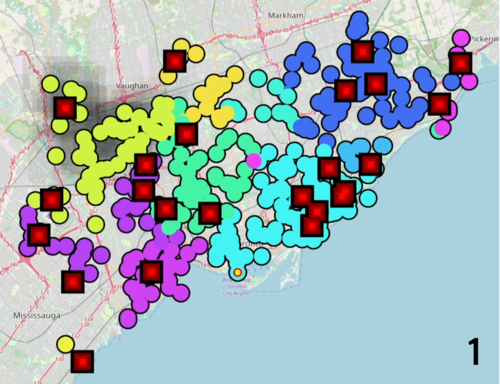
\includegraphics[width=\linewidth]{papers/ieee2022/img/snapshots/step-1.png-low.png}
  \end{subfigure}
  \hfill
  \begin{subfigure}[b]{0.39\linewidth}
    \centering
    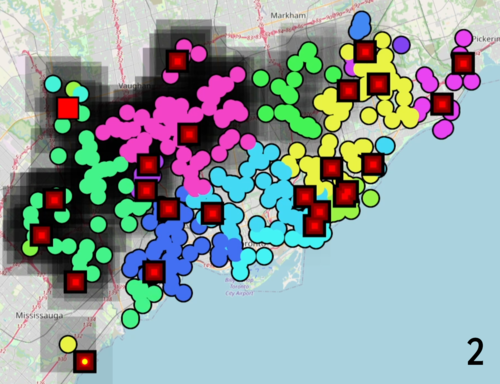
\includegraphics[width=\linewidth]{papers/ieee2022/img/snapshots/step-3.png-low.png}
  \end{subfigure}
  \\[0.15cm]
  \begin{subfigure}[b]{0.39\linewidth}
    \centering
    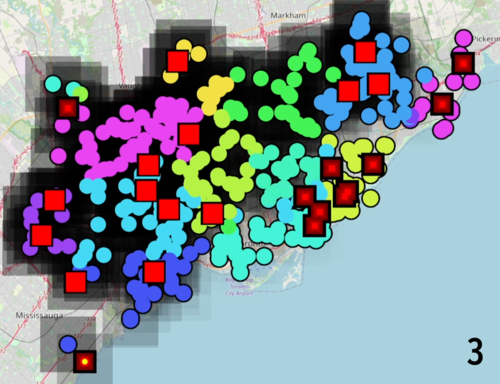
\includegraphics[width=\linewidth]{papers/ieee2022/img/snapshots/step-5.png-low.png}
  \end{subfigure}
  \hfill
  \begin{subfigure}[b]{0.39\linewidth}
    \centering
    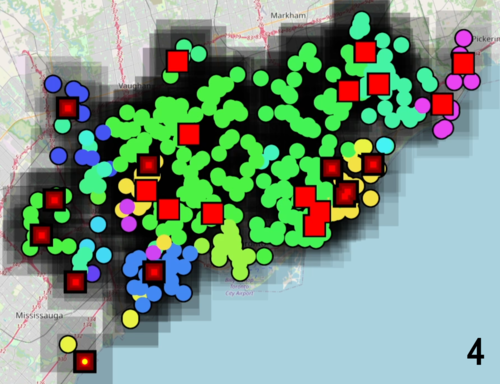
\includegraphics[width=\linewidth]{papers/ieee2022/img/snapshots/step-6.png-low.png}
  \end{subfigure}
  \caption[\casename{} simulation snapshots]{
    Subsequent simulation snapshots (left-to-right, top-to-bottom) of \casename{}.
    Darker shadows indicate heavier rain.
    Black squares with a small red dot are unalerted fire stations,
    when at least an alert reaches them, their dot changes to a large red square.
    Circles represent gauges;
    their colours map the \acp{dd} they are subject to when measuring rainfall intensity.
    A video of a complete simulation run is available at \url{https://bit.ly/3zysMOV}.
  }
  \label{fig:simulation-plots}
\end{figure}

\subsection{Results and discussion}\label{s:result-and-discussion}
\Cref{fig:simulation-plots} shows
that, when conditions change, \acp{dd} adapt by
changing their shape and extension to track the underlying phenomenon coherently;
in response to heavy rain,
close-by stations get appropriately alerted.
%
The system macroscopically tracks the underlying phenomena:
more operators get alerted when (\Cref{fig:simulation-charts})
and where (\Cref{fig:risk-evolution})
there are peaks in the signal.
%
However, even in response to similarly high peaks
the system may decide to allocate less or more resources to manage them:
differences are primarily due to the system detecting different base risks
(due to the altitude)
or the event being strictly local.
% \revise{
% Additionally,
% \Cref{fig:risk-evolution} shows that the alerted zones spatially track the evolution of the risk
% (as evaluated by an oracle using both altitude and current rainfall). 
% Indeed, the alarms follow the risky zone, 
%  approximating the maximum risk evaluated with an oracle.}

We now give some remarks to better contextualize the contribution.
%
Regarding applicability and generality,
 we observe that \acp{cct} and partitioning into \acp{dd}
 enable addressing several kinds of applications 
 in domains like 
 computing ecosystems,
 \acp{wsn},
 \ac{iot} and smart city,
 and multi-robot/multi-agent systems---cf. the surveys in~\cite{DBLP:journals/fgcs/PianiniCVN21,DBLP:journals/jlap/ViroliBDACP19}.
%
Details on quantitative cost/performance considerations on this kind of paradigm,
 can be found in~\cite{DBLP:journals/fgcs/PianiniCVN21,DBLP:journals/eaai/CasadeiVAPD21}: 
the focus of this article is on programming abstractions for \ac{cpsw}
 following a language-based software engineering approach~\cite{DBLP:journals/scp/Gupta15}.

\begin{figure*}[t]
  \begin{subfigure}[b]{0.49\linewidth}
    \centering
    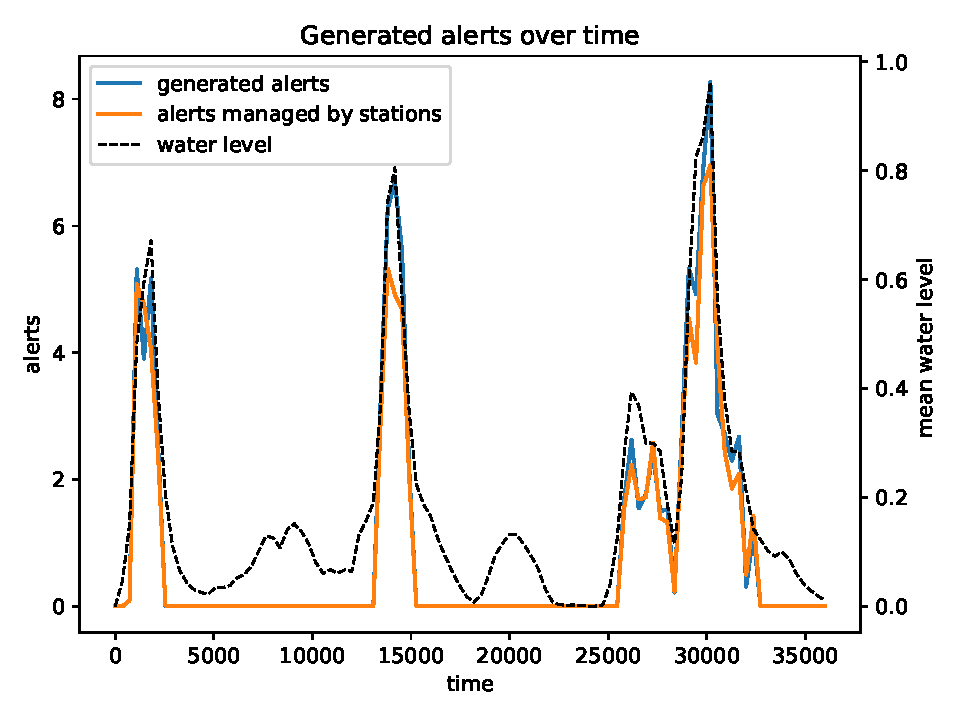
\includegraphics[width=\linewidth]{papers/ieee2022/img/charts/danger-and-managed.pdf}
  \end{subfigure}
  \hfill
  \begin{subfigure}[b]{0.49\linewidth}
    \centering
    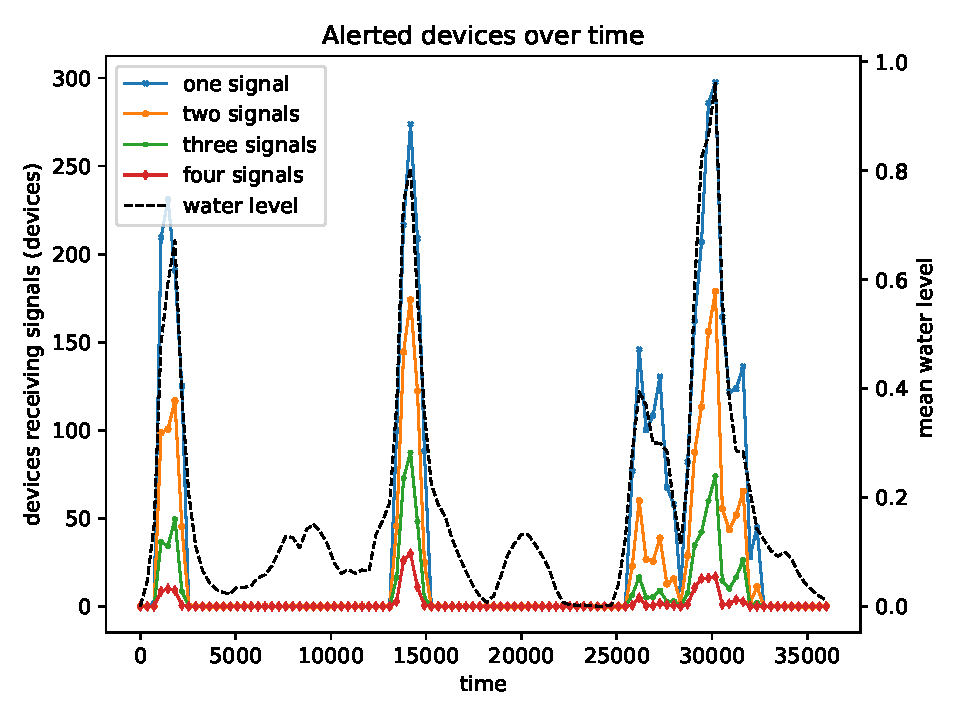
\includegraphics[width=\linewidth]{papers/ieee2022/img/charts/danger-evolution.pdf}
  \end{subfigure}
  \caption[\casename{} simulation]{
    Simulation results, showing, with time, the average rainfall intensity (dotted black line),
    the number of operator stations receiving alerts (left)
    and the breakdown by number of alerts received per station (right).
  }
  \label{fig:simulation-charts}
\end{figure*}
\begin{figure*}[t]
  \begin{subfigure}[b]{0.49\linewidth}
    \centering
    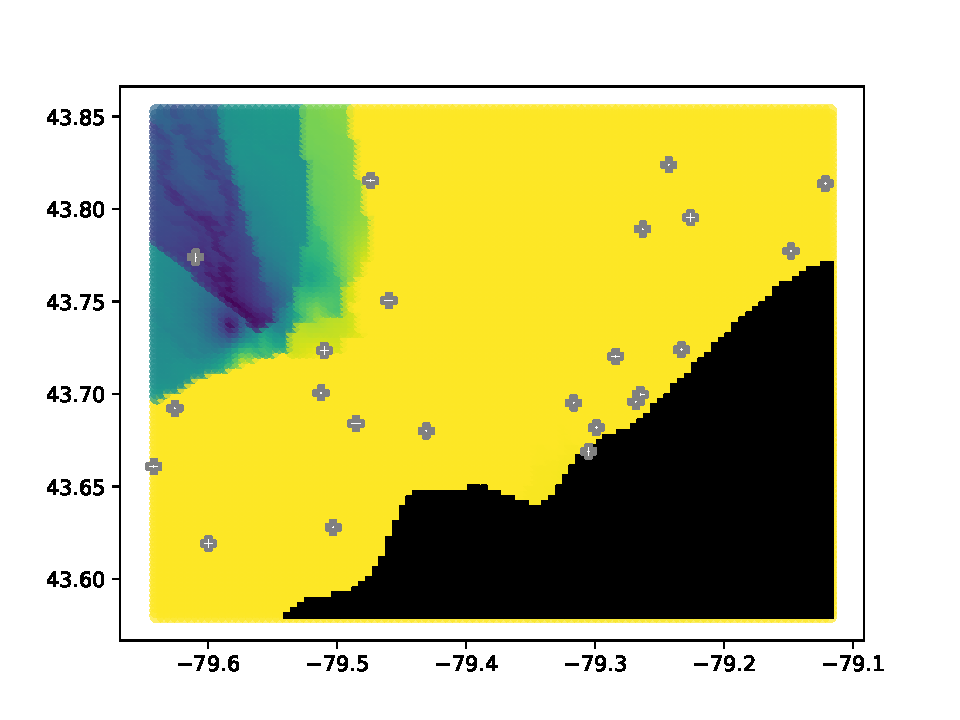
\includegraphics[width=\linewidth]{papers/ieee2022/img/charts/100.pdf}
    \subcaption{}
  \end{subfigure}
  \hfill
  \begin{subfigure}[b]{0.49\linewidth}
    \centering
    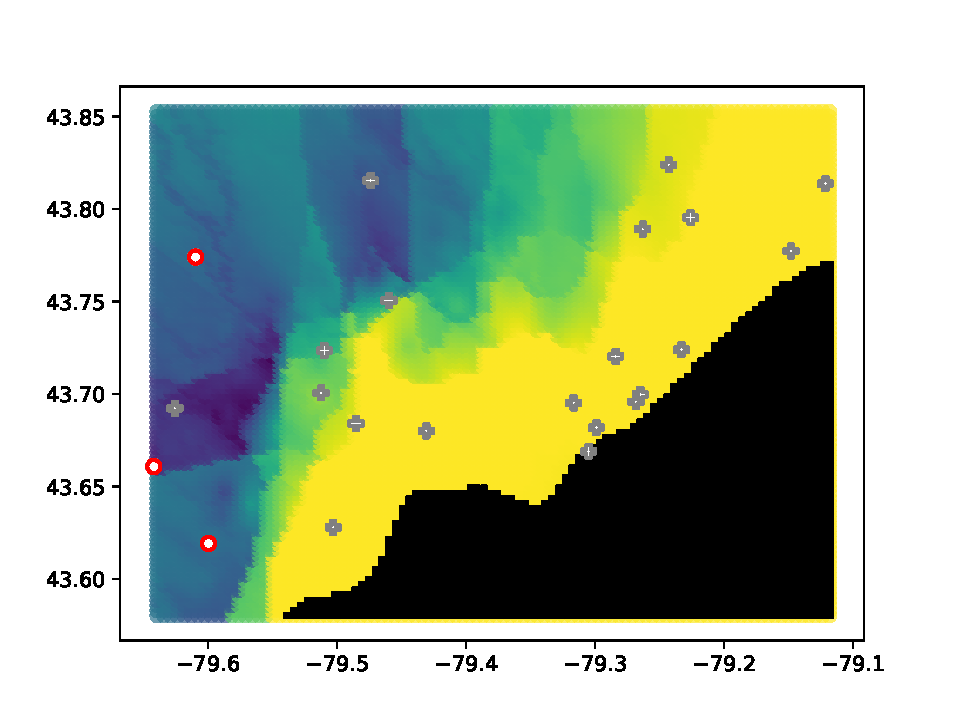
\includegraphics[width=\linewidth]{papers/ieee2022/img/charts/800.pdf}
    \subcaption{}
  \end{subfigure}
  \\[0.15cm]
  \begin{subfigure}[b]{0.49\linewidth}
    \centering
    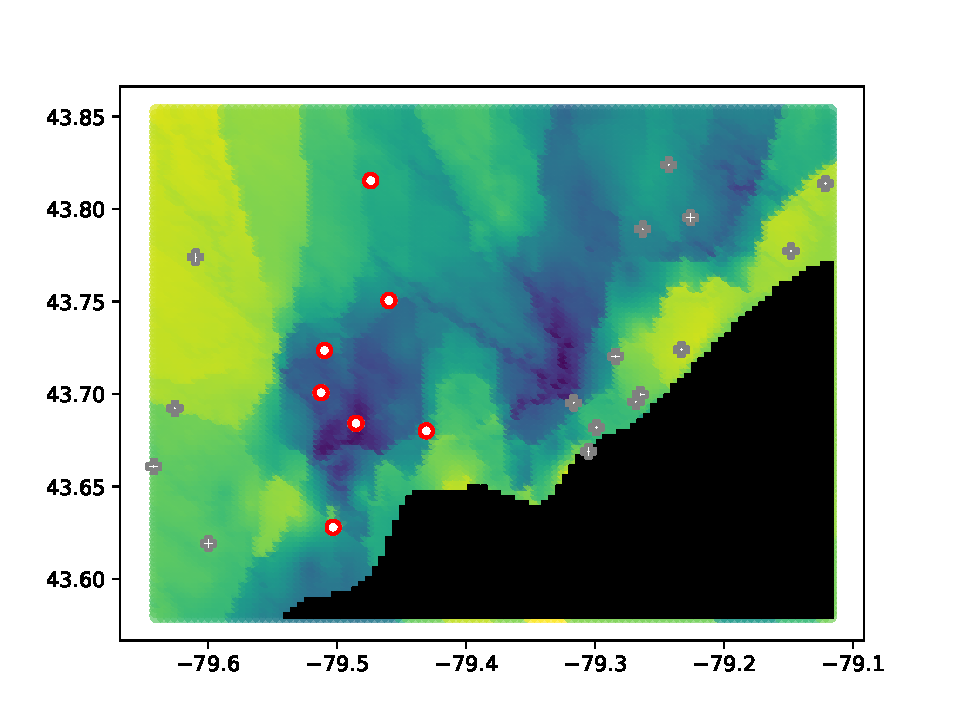
\includegraphics[width=\linewidth]{papers/ieee2022/img/charts/1500.pdf}
    \subcaption{}
  \end{subfigure}
  \hfill
  \begin{subfigure}[b]{0.49\linewidth}
    \centering
    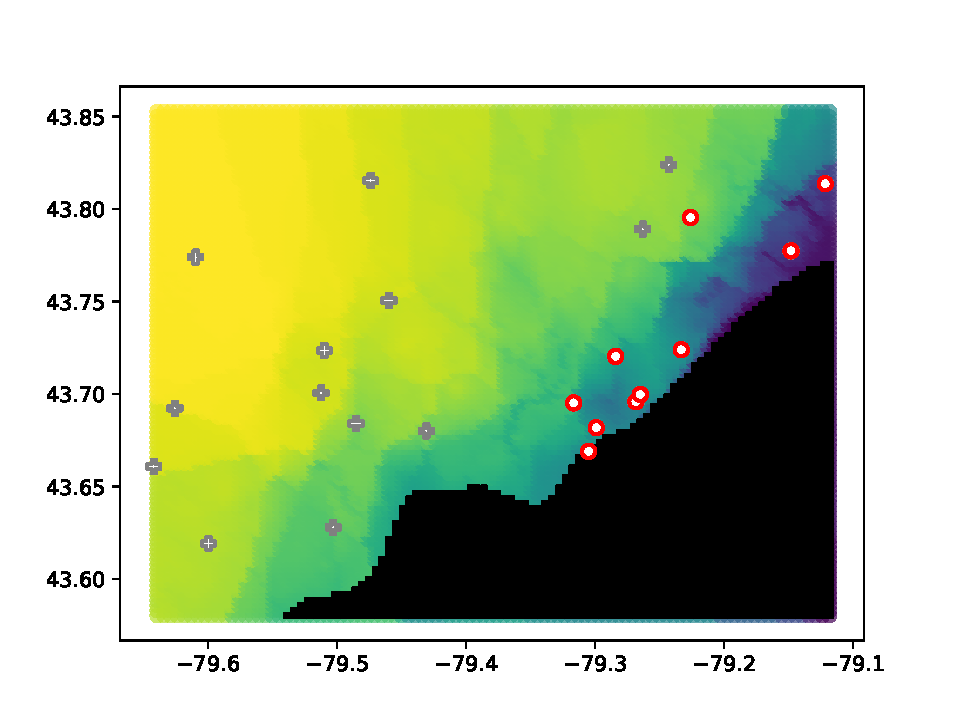
\includegraphics[width=\linewidth]{papers/ieee2022/img/charts/2200.pdf}
    \subcaption{}
  \end{subfigure}
  % \begin{subfigure}[c]{\linewidth}
  %   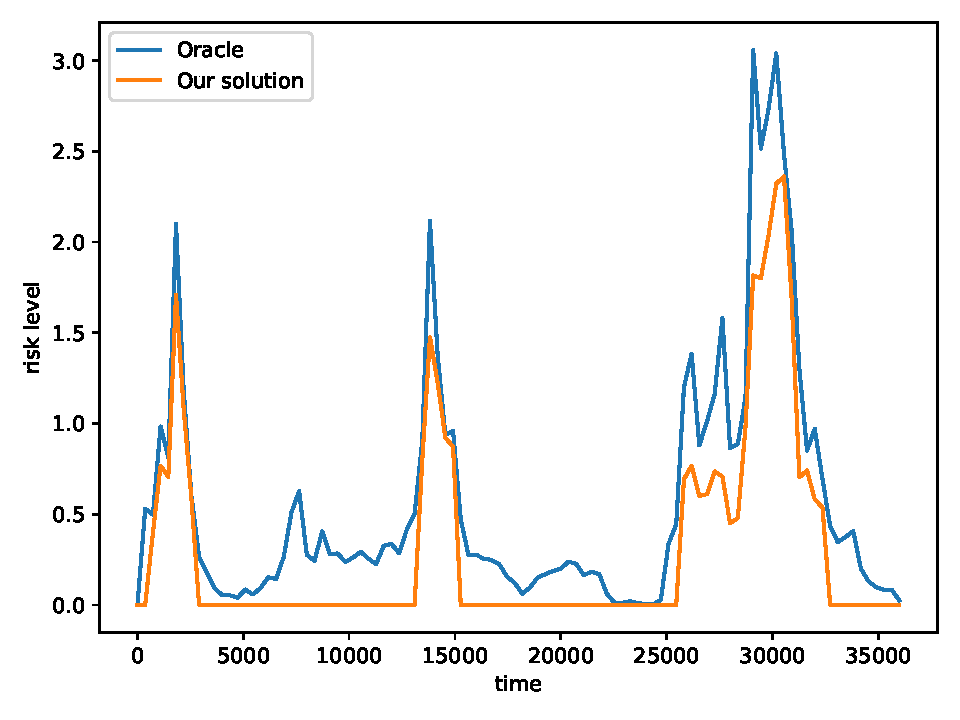
\includegraphics[width=\linewidth]{papers/ieee2022/img/charts/risk-oracle.pdf}    
  % \end{subfigure}
  \caption[\casename{} risk evolution]{
    \revise{
      Ability to track the risk spatially.
      Charts show risk (the darker, the higher) as estimated in real-time by an oracle using altitude and rainfall intensity.
      Stations are depicted with a red circle, and those alerted are filled in white.
      Solid black areas are non-land.
      Alerted stations are indeed those closest to the zones of the highest risk.
  }}
  \label{fig:risk-evolution}
\end{figure*}

\section{Final Remarks}\label{sec:conc}

%\meta{
%BUDGET: ca. 250 words
%% CURRENT: 226 words
%}
Mechanisms based on decentralization and self-organization
 are intensely researched
 and expected to play crucial roles in 
 next-generation applications
 involving \ac{cpsw}.
%
In this work,
 to turn decentralized activities into actionable notions,
 we propose a high-level programming model
 for situation recognition and action
 that originally integrates 
 recent developments
 in collective adaptive computing.
%
The idea is to expose a declarative \ac{api}
%  providing a structure
%  for the application logic of services 
%  that involve
featuring
 \emph{(i)} concurrent collective tasks which overlap in space
 and
 \emph{(ii)} non-overlapping decentralization domains
 with inner information flows-based feedback loops.
%
We implement the \ac{api} in Scala
 by mapping \acp{cct} and \acp{dd}
 to \scafi{} aggregate computations,
 then show the approach's effectiveness
 through a case study in flood monitoring and control.
%
Results show that programs expressed declaratively through the \ac{api}
%  when played collectively,
yield \acp{dd}
that can adapt to properly handle distributed monitoring and action.

This work focused on designing and programming 
 decentralized systems.
%
We believe that this level of control 
 is instrumental for properly structuring
 collective adaptive behaviour
 to steer desired emergents.
%
Building upon these foundational abstractions, 
 it becomes feasible to develop more intricate, high-level, and domain-specific constructs. 
 Towards this direction, in the following chapter, we introduce MacroSwarm, 
 a macro-programming API tailored for swarm-like system steering and control.